% -*- coding: utf-8 -*-


\chapter{IPv4がこの先生きのこるには}
% * (アスタリスク)付きの \chapter* コマンドは原則不可とする

\begin{flushright}
 yuyarin % ペンネーム
\end{flushright}

\section{はじめに}

\lettrine{イ}
ンターネットの主要技術であるIPv4というプロトコル.その中で個体識別子として使われるIPv4アドレスは32bitで表現され数は約42億個である.
かつては「無限アドレスだぜヒャッハー」と湯水のように消費されていたのだが,70億もの人間が社会インフラとしてインターネットを必要としている
今となっては,このアドレスの数が全く足りなくなってしまっているのだ.
IPv4アドレスの新規割り当てはほぼ終了しており,IPv4アドレスは「枯渇」したと表現されている.

そこで出てくるのがIPv6である.もちろんIPv4の失敗を踏まえて色々な改良は施されているが,なんといっても128bitのアドレス空間が魅力である.
国内主要ISPのバックボーンは既にIPv6に対応できており,一部のISPでは利用可能になっているが,中小ISPなどではまだ利用できない.

RFC2460にてIPv6の仕様が発表されたのが1998年なので,既に14年が経っているのだが,未だに普及していないのだ.
IPv6に対応するためにはお金がかかるので,ISPもICP\footnote{Internet Content Provider}もお互いにIPv6対応しない限りメリットがなくデッドロックに陥っているのだ.

さすがにこのままではダメだということで,先の2012年6月6日にはWorld IPv6 Launchとして,
Googleを筆頭に世界中の主要サイトがIPv6を恒久的に有効にするという取り組みが行われた.

こうして徐々にデッドロックが解けてIPv6への対応が進んでいき,IPv4アドレスの枯渇がそれを更に加速させるだろう.
そしていずれIPv6が主要のプロトコルになりIPv4は古の技術として扱われるようになる未来が来るだろう.
だがしかし,すべての通信がIPv6に対応できるまで,我々はアドレスが枯渇しているIPv4を必死に「延命」させなければならないのだ.

前置きが長くなったが,この章ではそんな「IPv4延命技術」を紹介しようと思う.

\section{IPv4延命技術概観}

枯渇によってIPv4アドレスの割り振りを受けられなかったISPにおいて,顧客に割り当てるIPv4グローバルアドレスが
無くなってしまうというシナリオが,今後実際に起こるだろう.というか起きてる.
この時に必要になるのは\textbf{顧客間でIPv4グローバルアドレスを共有する}方法である.
IPv4アドレスの共有にはNAT\footnote{実際にはNAPTだが以降NATと呼ぶことにする}が使われる.

主要な技術をNATの場所とIPv4パケットのトランスポート方法で分類した表を表\ref{yuyarin-nat-transport}に示す.

\begin{table}[htbp]
\begin{center}
\begin{tabular}{c|ccc} \hline
 & IPv4ネイティブ & \multicolumn{2}{c}{IPv6トランスポート} \\
 & & カプセル化 & トランスレーション \\\hline
CPEでNAT & いまここ & MAP-E(旧4rd) & MAP-T(旧dIVI) \\
ISPでNAT & CGN & DS-Lite & 464XLAT \\\hline
\end{tabular}
\end{center}
\caption{NATの場所とトランスポート方法によるIPv4延命技術の分類}
\label{yuyarin-nat-transport}
\end{table}

\subsection{IPv4ネイティブ方式}

現在のIPv4ネットワークではCPE\footnote{Customer Premises Equipment},いわゆるご家庭のルータでNATをしている.
これも1家庭1アドレス共有という1つのアドレス節約術であり,実は既にこの延命戦は始まっているのだ.
これに更にISP側でNATを重ねることで複数の家庭で1つのグローバルアドレスを共有するのがCGN(Carrier Grade NAT)である\footnote{表ではISPでNATとしているが,実際にはCPEとISPの両方でNATを行うことになる}.

\subsection{IPv6トランスポート方式}
それに対してCPEにIPv6アドレスを割り当て,そのIPv6を利用してISP網内のIPv4バックボーンまでIPv4パケットを通す方法がある.
これはIPv6の使い方によってカプセル化とトランスレーションに分けられる.
カプセル化はいわゆるトンネルのことで,CPEとISPの間でIPv4 over IPv6トンネルを張り,IPv4パケットをIPv6パケットのデータとして運ぶ.
トランスレーションではIPv4パケットをIPv6区間を通る間だけIPv6パケットに変換する.

\begin{figure}[htbp]
 \begin{minipage}{0.5\hsize}
  \begin{center}
   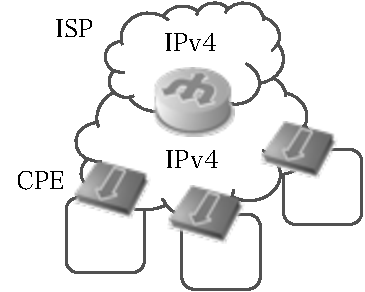
\includegraphics[bb=0 0 175 140,width=40mm]{./yuyarin/cgn.pdf}
  \end{center}
  \caption{IPv4ネイティブ}
  \label{fig:one}
 \end{minipage}
 \begin{minipage}{0.5\hsize}
  \begin{center}
   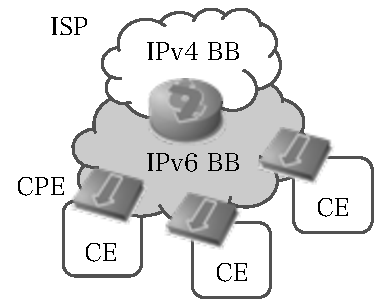
\includegraphics[bb=0 0 175 140,width=40mm]{./yuyarin/v6transport.pdf}
  \end{center}
  \caption{IPv6トランスポート}
  \label{fig:two}
 \end{minipage}
\end{figure}

これらは更にNATをする場所によって分類できる.
CPEでNATして,プライベートアドレスからグローバルアドレスへ変換した後,IPv6でカプセル化するのがMAP-E(かつての4rd),トランスレーションするのがMAP-Tである.
プライベートアドレスのIPv4パケットをIPv6でカプセル化してISP網内へ運んだ後,ISP側でNAT(CGN)してグローバルアドレスへ変換するのがDS-Lite(Dual Stack Lite),
プライベートアドレスのIPv4パケットをIPv6パケットにトランスレーション(NAT46)して,ISP側でNAT(NAT64)するのが464XLATである.
これらのIPv4グローバルアドレスは複数のCPEで同じ物が使われる.いくつのCPEで共有するかが設計のパラメータとなる,だいたい目安としては256程度である.

\section{ステート管理のお話}

\subsection{CGNのNATの問題}

NATの根底にある設計思想はアドレスだけでは識別子が足りないのでポート番号も識別子に使ってしまおうというものである.
NATでは(内部アドレス,内部送信元ポート,外部アドレス,外部送信元ポート)というバインディングをセッション情報として一定期間保持している.
そうしないと外から戻ってきたパケットを中の誰に送って良いのかわからなくなるからである.

CGNでは何千という家庭の通信をNATしなくてはならないので,NATのセッションデータベースは巨大なものになり生成頻度も高くなる.
ISPはユーザの通信を最低限90日間は保存しなくてはならないのだが,この時にNATのデータベースも併せて保存しておかないと
通信元の顧客が特定できなくなってしまう.

これらの処理はソフトウェアで行う必要があるためネットワーク機器からすれば意外と重い処理なのだ.
顧客数をnとすると定数項が大きい$\mathrm{O}(n)$の仕組みなのだがネットワーク業界ではこれはスケールすると言わなかったりする.

\subsection{IPv6トランスポート方式でのCPE特定の問題}

DS-Lite以外のIPv6トランスポート方式ではISPからCPEへIPv4パケットを送ろうとした時に,
どのIPv6アドレスのCPEに対してパケットを送るのかを特定しなければならない.
NATに非常によく似た状況であるのだが,IPv6のアドレスの長さを生かした工夫がされている.

MAPではIPv4アドレスとポート番号が決まればIPv6アドレスが相互に一意に定まるような「ルール」を決めてアドレス変換を行う,
Stateless Address Mapping(SAM)という方式を採用している.
ルールさえ各機器で共有してしまえばCPEを特定するためのデータベース(ステート)の管理をする必要がないのだ.
464XLATではRFC6145のStateless IP Translationを行なっており,こちらもステートを持たない.

この仕組みは顧客数nに対して定数オーダー$\mathrm{O}(1)$で処理できるために良くスケールする.
ISP側に置く設備1つに対して帯域が許す限り多くのCPEを収容しても問題ないのだ.

\subsection{ISP側NATにおける可用性の問題}

\begin{figure}
\centering
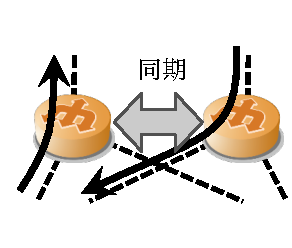
\includegraphics[bb=0 10 140 109,width=5cm]{./yuyarin/cgn-nat.pdf}
\caption{行きと帰りで違う箱を通るパケットと必死で同期するNAT箱}
\end{figure}

ISPでは当然ネットワークの冗長性を確保しなくてはならない.
ISP側でNATする技術については,2台の巨大NAT箱を置かなくてはならないのだ.

Act-Standby構成の場合,故障した時に即座にStandby機を起動して故障した機器からNATのセッションデータベースを受け取らなくてはならない.
故障しているのにそのようなことはできるはずがないので,当然ながらAct-Act構成になる.

IPネットワークでは往路と復路が必ずしも一致しない.NAT箱1を通って出ていったパケットの応答がNAT箱2に戻ってくることは,当たり前に起こりうることである.
よって2台のNAT箱は常にNATの巨大なセッションデータベースを同期し続け無くてはならないのだ.

もちろん非常に大変な処理なのだが,そこは力技でなんとかする感じである.

\section{結局どの技術がイケてるのか?}

\subsection{CGN}
スケールもしないし泥臭いので技術的には大変な割にダサい.
でも既存の家庭用ルータには手を入れずにISPに設備を置くだけでよい.
ハイスペックな機器があって,収容するCPEの数を上手に設計して,その分お金をかければなんとかなるのかもしれない.

\subsection{MAP-E(4rd), MAP-T}
MAPは技術的な面では非常にイケている.
ステートレスなアドレス変換を行うため定数オーダーでスケールところが非常に素晴らしい.

カプセル化をする場合はMTUの問題とフラグメントの問題が発生する.
実装面での負荷は高いが既存のMAP(4rd)実装ではこの点を既にクリアしている.
トランスレートする場合はIPv4の属性がIPv6に変換された時点で失われてしまう.

しかしながらデプロイが非常に難しい.
NTTのホームゲートウェイやBuffaloやNECのルータなど家庭用ルータにMAPの複雑な実装を入れなくてはならない.
ビジネス的な視点で見るとこれがとてつもなく高価になってしまうのだ.

\subsection{DS-Lite}
ISPでNATするのでCGN同様にスケーラビリティはない.
CPEにも機能を入れなくてはいけない.
あまりイケてない.

\subsection{464XLAT}
ステートフルトランスレーション(RFC6146)とステートレストランスレーション(RFC6145)の組合せで作られていて非常に美しい.
NAT64に始まるトランスレーション技術の最終形態とすら思える.

しかしやはりISP側でNATをしてステートを持ってしまうためスケールしない.
また各家庭のCPEに機能を追加する必要が出てくる.
今のところCPE(CLAT)ではNEC-ATなどの実装がある.
ISP側の機器(PLAT)はNAT64のため既に多くのベンダで実装が行われている.

\section{おわりに}

技術的にはMAPや464XLATがイケてるのだけれども,ビジネス的な面ではCGNでないとデプロイできないだろう.
とはいっても今回の記事で紹介したのはひとつの切り口であって,他にも語れなかった要素があるので,
他の技術も活躍できる場所が多いにあるのだ.結局は適所適材なのである.

アプリケーションを開発する人には,今後このように家庭間でのアドレス共有ということがISPで行われることを知ってもらいたい.
もはやIPアドレスだけでは誰かを特定できないのだ.
1つのIPアドレスでのBANが何千世帯に対して影響することが今後起こりうるのだ.
2ちゃんねるでプロバイダごとアク禁を食らったかのようなことが,いとも容易く起きてしまうのだ.

アドレスが枯渇したIPv4を我々はこのようなアドレス共有技術を用いてちまちまと延命していかなくてはならない.
自律分散システムであるがゆえに,地デジのように「今日でアナログ放送は終わりです」ということはできない.

IPv4はこの先生きのこらなければならず,そのためにはこうした技術や仕組みを考えて,標準化して,
製品に組み込んで,設計をして,お金をかけてリアルなインターネットにデプロイしなくてはならないのだ.

とっくの昔から,インターネットが止まると人が死ぬ時代になってしまっている.
ネットワークオペレータの戦いは終わらない.
